%Projects
%--------
%
%An essential part of this course are the take-home projects.
%
%Instructions for the take-home exams:
%
% Reports can be done individually or in groups of two. However, reasonably open
% discussions of the assignments with other students in this course are
% acceptable, but must be acknowledged in the report. The reports should consist
% of two to five pages plus supplementary graphs, tables, program listings, etc.,
% and should be organized as follows:
%
% Introduction and Problem Background. Briefly describe the general problem you
% want to solve and why a numerical or computational solution (as opposed to an
% exclusively analytical solution) is required.
%
% Numerical Considerations. Briefly discuss the specific methods, software or
% algorithms you selected for this problem. Mention any specific features of
% MATLAB you exploited.
%
% Results.  Include a concise tabular or graphical presentation of the results.
% Every table and figure should have a caption and a title, and the axes of every
% plot should be clearly marked, so that the reader can understand the figures or
% plots without referring to the main text. All codes should be clearly
% documented, especially input and output parameters, if any, and a description
% of what the code does.
%
% Analysis. Include a solid discussion and analysis of the results presented.
% The discussion should address any difficulties you encountered, appropriate
% measures of performance (such as errors and computer time) and the apparent
% sources of error you observed.
%
% Lessons Learned. Elaborate a critical evaluation of the software you used. Make
% a list of the specific things you  learned by working out the assignment, both
% theoretical and practical issues.
%
% Acknowledgements. Mention discussions with other students or teachers, software
% downloaded from the web or  copied from a book, and any other relevant
% information you find fit to disclose.
%
% The grade you obtain will reflect whether or not you have correctly and
% efficiently solved the problem, and whether or not you adequately address the
% relevant theoretical and practical issues. A grade of 8-12 indicates work that
% is acceptable, contains only minor errors, but is otherwise unexceptional. A
% grade of 13-15 indicates work that is correct, especially efficient and well
% documented, addresses all the points mentioned above, and contains unusually
% clear outputs and a serious and thorough analysis of those outputs.
%
% The report may be written in Swedish or English. Include name(s), ID number(s)
% and e-mail(s).
%
% Please hand in the report on paper (not via e-mail) at a lecture or seminar, or
% else place it in the box marked FMNF05 at the bottom of the shelf located at
% the entrance of the right-hand side corridor (MH, ground floor). The first
% report will be collected at 12:00 on Feb 2, 2018. The second project will be
% collected at 12:00 on Feb 23, 2018. Any report handed in or placed in the box
% after this time will not be accepted.

\documentclass{article}

\usepackage[utf8]{inputenc}
\usepackage[T1]{fontenc}
\usepackage{gensymb}
\usepackage{amsmath}
\usepackage{graphicx}

\begin{document}

\begin{center}
  {\small FMNF05 - Computational Project 1} \\
  {\Large\textbf{Numerical Crime Scene Investigation}} \\
  \vspace{0.4cm}
  \today\\
  \vspace{0.2cm}
  Stefan Eng \texttt{<atn08sen@student.lu.se>} \\
  \vspace{0.4cm}
  {\Large ---} \\
\end{center}

\section*{Introduction}

  \subsection*{Data}

  $T_{body}(\textrm{20:00}) = 32.0{\degree}C = T_{body}(0)$\\
  $T_{body}(\textrm{21:00}) = 29.5{\degree}C = T_{body}(1)$\\
  $T_{body}(t_{death}) = 37.0\degree{C} $ \\

  \noindent
  $T_{office}(\textrm{16:00}) = 22.0{\degree}C = T_{office}(0) $\\
  $T_{office}(t) = 22.0{\degree}C + 0.5{\degree}C \cdot t $\\

  \noindent
  Newtons law of cooling, $k$ = positive constant of proportionality: \\
  $T_{body}'(t) = -k(T_{body}(t) - T_{office}(t))$\\

  \noindent
  Problem: determine $t_{death}$ in order to check Sutherlands alibi.

\section*{Task 1}

  Show that the solution to: \\
  \hspace*{1cm}
  $T_{body}'(t) = -k(T_{body}(t) - T_{office}(t))$ \\
  given: \\
  \hspace*{1cm}
  $T_{office}(t) = 22.0{\degree}C + 0.5{\degree}C \cdot t $ \\
  is: \\
  \hspace*{1cm}
  $T_{body}(t) = 22 + 0.5t - \frac{1}{2k} + c\mathrm{e}^{-kt}$ \\

  \noindent
  $T_{body}(t) = 22 + 0.5t - \frac{1}{2k} + c\mathrm{e}^{-kt}$ \\
  $T_{body}'(t) = 0.5 -kc\mathrm{e}^{-kt}$ \\

  \noindent
  \begin{align*}
    T_{body}'(t) &= -k(T_{body}(t) - T_{office}(t)) \\
    0.5 -kc\mathrm{e}^{-kt} &= -k(22 + 0.5t - \frac{1}{2k} + c\mathrm{e}^{-kt}
    - 22 - 0.5t) \\
    0.5 -kc\mathrm{e}^{-kt} &= -k(-\frac{1}{2k} + c\mathrm{e}^{-kt}) \\
    0.5 -kc\mathrm{e}^{-kt} &= 0.5 - kc\mathrm{e}^{-kt} \\
  \end{align*}


\section*{Task 2}

  Show that given $T(0) = 32.0$ and $T(1) = 29.5$ results in: \\
  $T(t) = 22 + 0.5t - \frac{1}{2k} + (10 + \frac{1}{2k})\mathrm{e}^{-kt}$ \\

  \noindent
  \begin{align*}
    T_{body}(t) &= 22 + 0.5t - \frac{1}{2k} + c\mathrm{e}^{-kt} \\
    T_{body}(0) &= 22 - \frac{1}{2k} + c\mathrm{e}^{0} \\
    32 &= 22 - \frac{1}{2k} + c \\
    10 &= -\frac{1}{2k} + c \\
    c  &= 10 + \frac{1}{2k} \\
  \end{align*}

  \begin{align*}
    T_{body}(t) &= 22 + 0.5t - \frac{1}{2k} + c\mathrm{e}^{-kt} \\
    T_{body}(1) &= 22 + 0.5 - \frac{1}{2k} + c\mathrm{e}^{-k} \\
    29.5 &= 22.5 - \frac{1}{2k} + c\mathrm{e}^{-k} \\
    7 &= - \frac{1}{2k} + c\mathrm{e}^{-k} \\
    7 + \frac{1}{2k} &= (10 + \frac{1}{2k})\mathrm{e}^{-k} \\
  \end{align*}

\section*{Task 3}

  \textbf{Task:}
  Construct a MATLAB algorithm that approximates the value of $k$ with an
  accuaracy of two decimal places using the bisection method. \\

  \noindent
  The task is equivalent to finding a root to the function:
  $ f(x) = 7 + 0.5x - (10 + 0.5x)\mathrm{e}^{-x} $.
  In order to use the bisection method, an intitial x-interval of $[a, b]$ must
  be choosen in such a way that $f(a) * f(b) < 0$, i.e. the interval brackets the
  root. Two such values are 0 and 1, which results in; $f(0) = -3$ and $f(1) >
  0$, which gives the initial values of $a=0$ and $b=1$.

  \begin{center}
    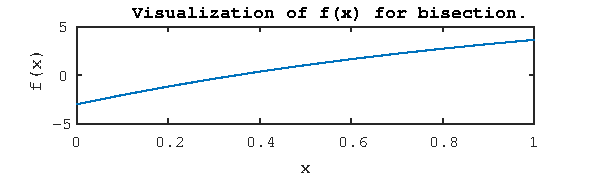
\includegraphics{figs/t3_check.pdf}
  \end{center}

  \noindent
  Running the $x_c =\ $\texttt{bisection} in MATLAB, with $a=0$, $b=1$,
  $\epsilon=0.5*10^{-2}$ and $Nmax=100$, produces $x_c = 0.34961$ with $f(x_c) =
  0.001940 \ ( < 0.5*10^{-2} )$ running 9 iterations.

\section*{Task 4}

  \textbf{Task:} Use a algorithm based on the fixed point method to appriximate
  $k$ to 6 decimal accuracy. \\

  \begin{align*}
     f(x) &= 7 + 0.5x - (10 + 0.5x)\mathrm{e}^{-x} = 0\\
     0  &= 7 + 0.5x - (10 + 0.5x)\mathrm{e}^{-x} \\
     - 0.5x  &= 7 - (10 + 0.5x)\mathrm{e}^{-x} \\
     x  &= -2(10 + 0.5x)\mathrm{e}^{-x} + 14  = g(x)\\
  \end{align*}

  $ g(x) = -2(10 + 0.5x)\mathrm{e}^{-x} + 14 $

\end{document}
